\documentclass[a4paper, 12pt]{article}
\usepackage[yyyymmdd]{datetime}
\usepackage{fontspec}
\usepackage{fontenc}
\usepackage{amssymb}
\usepackage{ulem}
\usepackage{cite}
\usepackage{multirow}
\usepackage{mathtools}
\usepackage{amsmath}
\usepackage{float}
\usepackage{graphicx}
%\usepackage{url}
\usepackage{hyperref}
\usepackage{caption}
\usepackage[svgnames]{xcolor}
\usepackage{xstring} % to define myund
\usepackage[lithuanian]{babel}
%\usepackage{lineno}
\graphicspath{ {images/} }

\usepackage{geometry}
\pagestyle{myheadings}
\geometry{
	left=2cm,
	right=2cm,
	top=2cm,
	bottom=2cm,
}
\pagenumbering{arabic}
\linespread{1.25}

\renewcommand{\dateseparator}{-}
\renewcommand{\abstractname}{Santrauka}
\renewcommand{\contentsname}{Turinys}
\renewcommand{\figurename}{Pav}
\renewcommand{\refname}{Literatūra}
\renewcommand{\tablename}{Lentelė}
\renewcommand{\listfigurename}{Paveikslėlių sąrašas}
\renewcommand{\listtablename}{Lentelių sąrašas}

\DeclareCaptionLabelFormat{numfirst}{#2~#1}
%\captionsetup[figure]{labelformat = numfirst, labelsep = period}
\captionsetup[figure]{labelformat = numfirst, labelsep = space}
\captionsetup[table]{labelformat = numfirst, labelsep = period}

\newcommand{\textblue}[1]{{\color{Blue}#1}}
\newcommand{\textred}[1]{{\color{Red}#1}}
\newcommand{\comment}[1]{\newline\textblue{#1}\newline}
\newcommand{\commentNL}[1]{\textblue{#1}\newline}
\newcommand{\commentMA}[1]{\newline\textred{#1}\newline}
\newcommand{\commentMANL}[1]{\textred{#1}\newline}
\newcommand{\pT}{p_{T}}
\newcommand{\DYtau}{\mathrm{DY}\!\rightarrow\tau\tau}
\newcommand{\DYee}{\mathrm{DY}\!\rightarrow ee}
\newcommand{\WJets}{W\! +\!\mathrm{Jets}}
\newcommand{\QCD}{\mathrm{QCD}}
\newcommand{\Data}{\mathrm{Data}}
\newcommand{\MC}{\mathrm{MC}}
\newcommand{\est}{\mathrm{est.}}
\newcommand{\emu}{e\mu}
\newcommand{\ET}{E_{T}}
\newcommand{\refeqq}[1]{(\ref{#1})}
\newcommand{\Lumi}{{\cal L}_\mathrm{int}}
\newcommand{\invfb}{fb$^{-1}$}
\newcommand{\invpb}{pb$^{-1}$}
\newcommand{\ltq}[1]{{\quotedblbase{}#1\textquotedblleft{}}}
\newcommand{\beq}{\begin{equation}}
\newcommand{\eeq}{\end{equation}}
\newcommand{\ttt}[1]{\texttt{#1}}

\def\myund#1{%
  \saveexpandmode\expandarg
  \IfSubStr{#1}{_}{%
   \StrSubstitute{#1}{_}{\_}}{#1}%
  \restoreexpandmode
}


\begin{document}

%\linenumbers

\title{Darbų dienoraštis}
\author{M.\ Ambrozas}
\date{\textit{Pradėta} 2018-10-09, \textit{Paskutinė versija} \today}
\maketitle
\pagebreak

\section{Spalio 9-10 d. -- CMSDAS ataskaitos taisymas}
\begin{itemize}
	\item Tikrinau, ar veikia neinteraktyvus skaičiavimas tier3 centre
	(prieš tai kelis kartus buvo išmetę klaidą, kad neįmanoma įrašyti atrinktų
	įvykių į failą, nes nėra tinkamo serverio, tačiau, kai pabandžiau paleisti
	tuos pačius skaičiavimus, tik su 100 įvykių kiekvienam procesui, viskas veikė
	normaliai) -- pabandžiau paleisti atskirus skaičiavimus su $WW$, $WZ$, $ZZ$,
	$tW$, $\overline{t}W$ procesais. Panašu, kad viskas suveikė normaliai, failų
	įrašymas buvo sėkmingas. Dar ko gero reikėtų pabandyti paleisti skaičiavimą
	su kitais procesais, kad galima būtų spręsti, ar ten buvo tik laikina problema
	su tier3 sistemomis, ar ši problema priklauso nuo bandomų įrašyti failų dydžio,
	ar nuo sistemos vykdomų skirtingų darbų skaičiaus ir pan.
	\item Trumpai peržiūrėjau \textit{DY working meeting 2018-06-22} skaidres
	(\url{https://indico.cern.ch/event/736672/contributions/3038893/
	attachments/1673244/2685121/DY_working_meeting_20180622.pdf}).
	Panašu, kad ten buvo naudojamas vienodas integruotas šviesis tiek $ee$, tiek
	$\mu\mu$ įvykiams, o pritaikius korekcijas (PU, Rochester (miuonams),
	track (miuonams), reco (elektronams) ID, iso (miuonams), trigger) nesutapimai
	tarp eksperimento ir modeliavimo siekia maždaug iki 5 procentų. Kadangi mano
	atveju taip nėra, trupmai užmečiau akį i mano korekcijų kodus (kuriuos paėmęs
	iš Kyeongpil Lee github saugyklos netaisiau) -- bent jau prie elektronams
	taikomų korekcijų nėra bandoma įvertinti trigerio efektyvumo. Taip pat skaidrėse
	vaizduojami PU pasiskirstymai neatrodo panašūs į mano turimus (skaidrėse
	esantys pasiskirstymai atrodo panašūs į 2015 metų duomenų pasiskirstymą, tik
	PU vertės vidurkis didesnis, o mano turimi pasiskirstymai turi kažką panašaus
	į lokalų maksimumą ties mažesnėmis PU vertėmis). Taip pat ir po PU korekcijos
	vaizduojama PU pasiskirstymo Data/MC kreivė savo forma atrodo labai nepanaši
	į mano (nors taip galbūt gali būti ir todėl, kad nežinau, ar savo grafikuose
	atvaizduoju \ltq{tikrą} eksperimentinį PU pasiskirstymą: jį pavaizduoju pagal
	failą, kuriuo naudojantis skaičiuojama modeliuotų įvykių PU svorio vertė, nes
	eksperimentiniuose dydžiuose kintamasis \ttt{nPileUp} visur duoda 0.
	\textbf{Reikia pasidomėti, kaip daromos tos korekcijos ir pabandyti pasitaisyti
	kodus, kad viskas būtų įskaitoma kaip reikia (tam taip pat ko gero reikės
	sutikrinti, ar korekcijų skaičiavimuose naudojamos failų versijos yra tinkamos)}.
	\item Pagal vadovo pastabas taisiau CMSDAS ataskaitą. Pagrindinės problemos buvo
	per daug bendrų, nieko konkretaus nepasakančių frazių vartojimas, per mažas
	asmeninės patirties perteikimas. Kad ką nors pamiršęs nepridaryčiau faktinių
	klaidų, užtrukau nemažai peržiūrėdamas iš naujo darytų užduočių skaidres,
	twiki puslapius ir pan.\ (visos užduotys gali būti rastos čia:
	\url{https://twiki.cern.ch/twiki/bin/viewauth/CMS/WorkBookExercisesCMSDataAnalysisSchool},
	paskaitų skaidres galima rasti čia: \url{https://indico.cern.ch/event/684249/timetable/#20180910})
\end{itemize}

\section{Spalio 12 d. -- CMSDAS ataskaitos taisymas}

\begin{itemize}
	\item Ant tier3 paleidau neinteraktyviai skaičiuoti su kitais procesais,
	kad patikrinčiau, ar problema tebėra.
	
	\textbf{UPDATE vakare:} paskaičiavau su procesais DYEE\_10to50, DYEE\_50to100,
	DYTauTau\_10to50, DYTauTau\_50to100, WJets, ttbar. Kol kas baigė skaičiuoti su
	Drell-Yan procesais, viskas veikė normaliai, WJets ir ttbar dar tebeskaičiuoja.
	Kita problema: kažkodėl po to, kai skaičiavimas baigiasi, HTCondor sistema vietoje
	to, kad mano paduotą darbą tiesiog užbaigtų (ir įvedus komandą condor\_q
	darbas būtų rodomas prie užbaigtų -- sekcijoje DONE), ji darbo vykdymą
	tiesiog pristabdo (rodo sekcijoje HELD). Galbūt taip gali būti dėl to,
	kad darbas nebūna atliekamas be jokių klaidų žinučių -- kažkodėl klaidų išvestyje
	gaunu tokį pranešimą:
	
	\ttt{WARNING: In non-interactive mode release checks e.g. deprecated releases,
	production architectures are disabled.\\
	**** Following environment variables are going to be unset.\\ SCONS\_LIB\_DIR}
	
	Nežinau, ką jis reiškia, bet skaičiavimui lyg ir netrukdo.
	\item Bandžiau dar kartą įsitikinti, ar tikrai eksperimentiniuose duomenyse
	dydis \ttt{nPileUp} visada yra lygus nuliui. Įsitikinau, kad taip, bet pastebėjau,
	kad taip pat duomenyse yra saugomas dydis \ttt{nVertices}, kuris eksperimentiniams
	duomenims jau nelygus nuliui. Tikrinau, kaip yra modeliuotuose duomenyse: ten taip
	pat yra dydis \ttt{nVertices}, bet šio dydžio pasiskirstymas nesutampa su
	\ttt{nPileUp} pasiskirstymu.
	\item Dar  porą kartų taisiau CMSDAS ataskaitą. Šį kartą pagrinde tai jau buvo rašybos, formulavimo
	arba minčių nuoseklumo klaidos.
	\item Taisiau duomenų naudojimo schemą ir pradėjau daryti duomenų saugojimo tier3 schemą.
\end{itemize}

\section{Spalio 16 d. -- CMSDAS ataskaitos taisymas}
\begin{itemize}
	\item Galutinai pataisiau CMSDAS ataskaitą.
	\item Paleidau skaičiuoti daug procesų ant tier3.
	
	\textbf{Update:} visus failus įrašinėjo tvarkingai, išskyrus DYEE\_M50to100 --
	ten išmetė daugybę žinučių, sakančių, kad neišeina sukurti šakų medžiui
	ir to medžio įrašyti į failą, bei siūlančių kode pirmiau apsibrėžti failą, o
	tik po to -- medį. Keista, nes aš taip ir darau.
	
	Taip pat visi procesai buvo sustabdyti (\ttt{held}) vietoje to, kad baigtų darbą.
	Įvedus į terminalą \ttt{condor\_q -analyze <darbo\_nr>} gavau atsakymą, kad taip yra
	dėl to, kad nesėkmingai yra sukuriamas rezultato išvesties failas, pavadinimu
	\ttt{RESULT}. Iš esmės, jame nieko nėra įrašoma ir jis man yra nereikalingas, tiesiog
	taip buvo parašyta pavyzdyje, kurį žiūrėjau, tad galbūt ištrynus atitinkamas eilutes
	klaidos nebeliks.
	
	Informaciją, apie HTCondor komandas radau čia:
	\url{http://research.cs.wisc.edu/htcondor/manual/v8.6/2_Users_Manual.html}
	
	\item Bandžiau sudėlioti duomenų laikymo tier3 centre schemą. Kažkaip atrodė natūralu
	į ją įkomponuoti ir mano \ttt{FileMgr} klasės dalis, kad eitų suprasti, kaip
	konkrečiai tie duomenys bus naudojami. Kadangi klasė šiek tiek skirtingais būdais
	laiko tikrų ir modeliuotų įvykių adresus, buvo gan sudėtinga sugalvoti, kaip kuo
	paprasčiau viską atvaizduoti. Pabandžiau padaryti dvi versijas -- vieną paprastesnę,
	kuri vaizduoja tik tai, kaip klasė pateikia modeliuotų įvykių adresus, ir kitą --
	sudėtingą, kur vaizduojami abu atvejai, bet tada schema pasidaro jau sunkiai suprantama.
	
	\begin{figure}
		\centering
		\label{fig:duomSchemSud}
		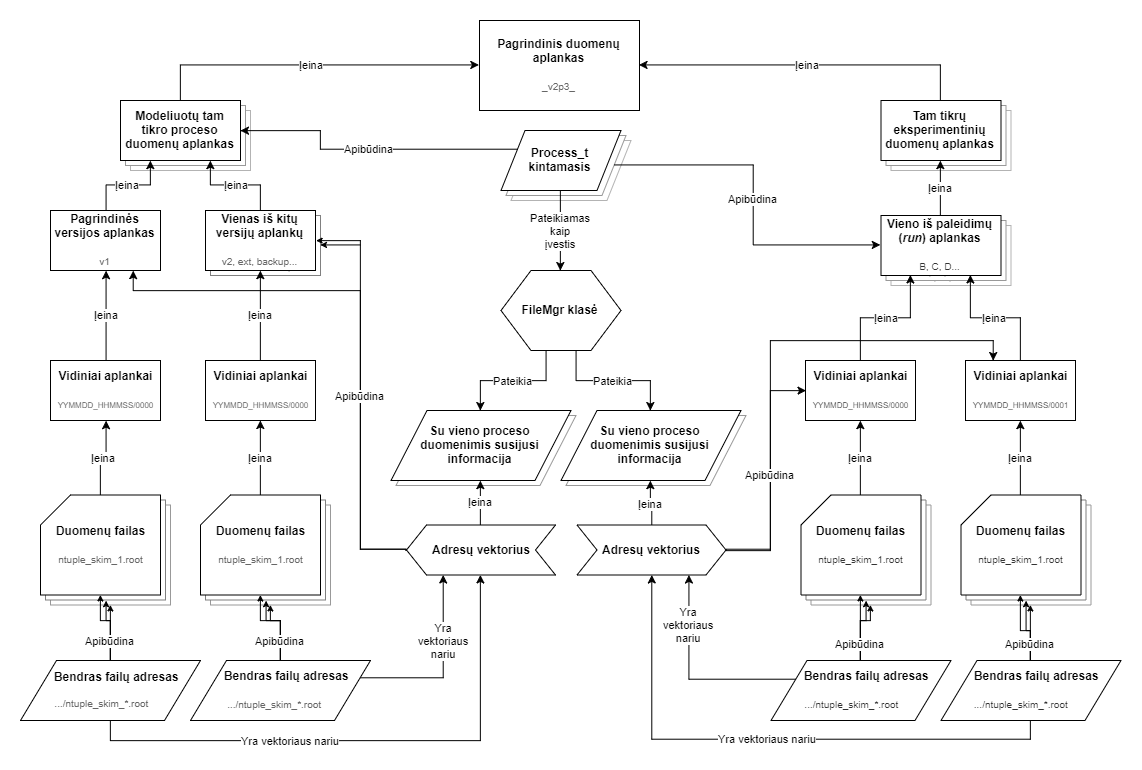
\includegraphics[width=\textwidth]{Duomenu_schema_10-16.png}
		\caption{Sudėtinga duomenų schema. Spalio 16 d. versija.}
	\end{figure}
	\begin{figure}
		\centering
		\label{fig:duomSchem}
		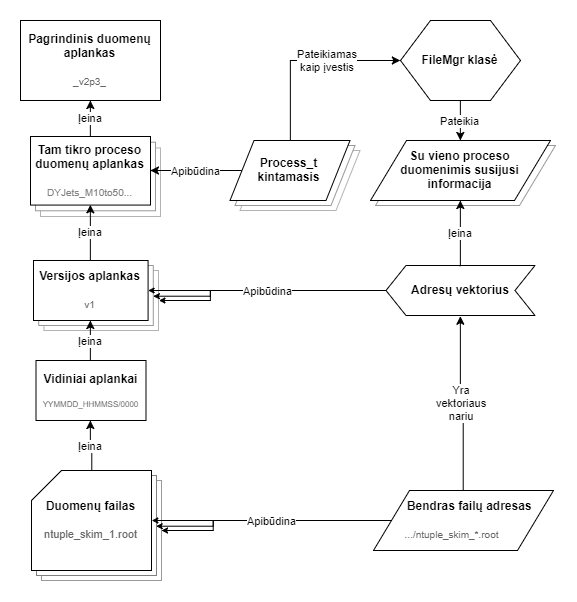
\includegraphics[width=0.7\textwidth]{Duomenu_schema_paprasta_10-16.png}
		\caption{Supaprastinta duomenų schema. Spalio 16 d. versija.}
	\end{figure}
\end{itemize}

\section{Spalio 17-18 d. -- reikalų tvarkymas}
\begin{itemize}
	\item Bandžiau peržiūrėti skaidres iš Spalio 16 dieną vykusių DY mokslinių
	grupių pristatymų. Spėjau peržiūrėti tik skaidres apie pirminį spinduliavimą
	(angl. \textit{Initial State Radiation -- ISR}). Galiu pasakyti, kad supratau
	nedaug.
	\item Gavau užduotį padaryti plakatą, kuriame būtų informacija apie vykdomą
	LMT projektą, kad jį būtų galima atspausdinti ir pakabinti. Plakatą padariau
	ir nusiunčiau administratoriui. Jis bandė įsiūlyti į plakatą pridėti savo
	vardus, pavardes, nuotraukas ir pan., bei išsispausdinti 10 plakatų ir juos
	pakabinti visur, kur tik įmanoma, bet mes su vadovu šiai minčiai nepritarėme.
	\item Šiek tiek bandžiau koreguoti duomenų schemą, bet nelabai spėjau.
	\item Ieškojau kompiuterio, kuris turėtų mano norimas specifikacijas
	(Intel 8 kartos procesorių, NVIDIA vaizdo plokštę, skaičių klaviatūrą, bent
	8 GB DDR4 RAM atminties ir pan.), ir kurį eitų nupirkti iš projekto pinigų
	(už ne daugiau, kaip 1000 eurų). Radau kelis variantus, nusiunčiau vadovui.
\end{itemize}

\section{Spalio 19 d. -- registracija į techninio studento praktiką, reikalų tvarkymas}
\begin{itemize}
	\item Iš naujo peržiūrėjau išsirinktų kompiuterių sąrašą, patikrindamas,
	ar jie atitinka ir vadovo pridėtus kriterijus (HDMI ir JR45 jungtys, matinis
	ekranas). Pakalbėję su vadovu nutarėme, kad reikėtų susidėlioti 5 kompiuterių
	sąrąša, kurie būtų daugmaž panašūs, ir kurie man tiktų ir tada pateikti
	administratoriui, kuris pažiūrėtų, ką galima padaryti (galima apklausti kelias
	įmones, už kiek jie parduotų tam tikrą kompiuterį ar kelis ir tada išsirinkti
	pigiausiai pasiūliusią įmonę), ir ar tikrai įmanoma iš projekto pinigų nusipirkti
	kompiuterį. Sąrašą sudariau, bet gavosi taip, kad visi 5 kompiuteriai iš sąrašo
	internete kainuoja šiek tiek virš 900 eurų, tad apsidraudimui (jeigu perkant per
	projektą įmonės prašytų daugiau, sudėliojau ir 5 pigesnių kompiuterių sąrašą
	(arti 900 eurų arba mažiau).
	\item Bandžiau pildyti registraciją CERN techniniam studentui. Iš visų siūlomų
	sričių išsirinkau taikomosios fizikos sritį (nes iš aprašymo mačiau, kad ten
	galima gilintis į detektorių fiziką, trigerius ir pan.). Kadangi ten reikėjo
	prisegti savo akademinius rezultatus įrodantį dokumentą bei buvo pateiktas
	įspėjimas, kad užpildžius paraišką daugiau dokumentų prisegti bus nebegalima,
	bijojau pildyti, kol neturėjau reikiamų dokumentų. Su vadovu pasitariau, kad
	ko gero ten galiu prisegti tiesiog savo universiteto diplomą (kurio kopiją jau
	ir taip turiu kompiuteryje), nes naujesnių pažymių dar nesu gavęs. Pildant
	paraišką reikėjo pateikti ir CV, kurį buvo galima pasirašyti internetinėje
	sistemoje \ltq{Indeed} ir ten tiesiogiai įkelti, tad taip ir padariau.
	Registracijoje reikėjo įrašyti savo veiklos patirtį susijusioje srityje (mano
	atveju tai gavosi detektorių fizika). Iš pradžių nelabai žinojau, ką ten rašyti,
	nes maniau, kad tokios patirties neturiu išvis, galbūt išskyrus tai, kad lankiau
	Christoph Schaefer paskaitas, tačiau vadovas mane pamokė, kad gebėjimas dirbti
	su linux operacine sistema, programuoti Python ir C++ kalbomis, ROOT žinios ir
	pan.\ jau yra su šia sritimi susijusi patirtis. Paraišką užpildžiau ir pateikiau,
	išsisaugojau, kaip ji atrodo ir sudėjau į PDF dokumentą, kad, jeigu kas nors
	kitas pildys vėliau, geriau žinotų, kaip ten viskas atrodo, ir galėtų lengviau
	užpildyti. Gavau laišką su nuoroda, į kurią bent vienas žmogus turi įkelti
	rekomendaciją. Nuorodą išsiunčiau vadovui bei dr. Gajdosik'ui.
	\item Paleidau nedidelį neinteraktyvų skaičiavimą ant tier3, kad pažiūrėčiau,
	ar nebesustabdo darbo, jeigu nebandau į kažkokį failą įrašyti rezultatų.
	
	\textbf{Suveikė} -- dabar darbas tiesiog baigiamas, kai baigiasi skaičiavimas.
	\item Ištryniau testinius HTCondor paleidimo kodus ir palikau pataisytus
	normalius. Pagal idėją turėtų veikti.
	\item Parašiau laišką Dalmin Pai ir KyeongPil Lee su klausimu, ar jie žino,
	kodėl mano \ttt{/xrootd/store/user/} aplankas tier3 centre man pasidarė
	\ltq{read-only}, ir kaip šią problemą galima būtų išspręsti. Greitai gavau
	atsakymą iš Dalmin'o, kad tier3 administratorius taip padarė specialiai visiems
	vartotojams, nes kažkoks studentas ištryninėjo svetimus failus. Taip pat paminėjo,
	kad taip yra tik laikinai, tačiau neaišku, kiek ilgai tęsis.
\end{itemize}

\section{Spalio 22 d. -- Schemos darymas, MuMu atrankos redagavimas}
\begin{itemize}
	\item Skaičiau DY mokslinių grupių pristatymų likusias skaidres. Pagalvojau,
	kad būtų verta patikrinti, ar taip pat vykdau įvykių atranką, kaip nurodyta
	Dalmin Pai skaidrėse. Pastebėjau, kad taip pat vykdau tik elektronų atranką,
	o miuonų reikia pakeisti (vietoje \ttt{TightMuon} kriterijaus naudojau
	\ttt{HighPtMuon} ir vietoje \textit{ParticleFlow} izoliacijos -- treko izoliaciją).
	Taigi pamodifikavau atrankos kodus. Taip pat papildžiau \ttt{SelectedX} klases
	kintamuoju \ttt{nVertices}, nes eksperimentiniuose duomenyse dydžis \ttt{nPileUp}
	nėra gaunamas.
	\item Pradėjau schemą daryti iš naujo, nes reikia į duomenų struktūrą pažvelgti
	iš toliau -- mažiau lįsti į detales, daugiau į pačią esmę (t.y., kad duomenys yra
	eksperimentiniai ir modeliuoti, jie yra savo esme skirtingi ir pan.).
\end{itemize}

\section{Spalio 23 d. -- schemų tvarkymas, kodų taisymas}
\begin{itemize}
	\item Tvarkiau spalio 22 d.\ pradėtą schemą. Iš vadovo gavau pastabų, kad ji
	turėtų būti dar bendresnė -- t.y.\ iš vis neturėtų būti kalbama apie failų
	struktūrą, tik apie pačią idėją (kad yra eksperimentiniai ir modeliuoti duomenys,
	ir kaip jie skiriasi). Taigi pradėjau daryti dar vieną schemą, kuri išsivystė į tris
	atskiras schemas. Tada padariau schemą, kuri vaizduoja, pagal kokią logiką skirstomi
	duomenys katloguose.
	
	\item Bandžiau ant tier3 HTCondor sistemos paleisti skaičiavimus su $\mu\mu$ 
	įvykiais -- kažkodėl išmeta \ttt{Break: Segmentation violation}. Tikrinau, kodėl
	taip gali būti. Nustačiau, kad kodas nulūžta tada kai bando inicializuoti
	\textit{Rochester} korekcijos klasę. Bandžiau ieškoti, kur bėda, bet atrodė, kad
	lyg ir viskas gerai. Paleidus kodą interaktyviai jis nenulūždavo. Tada pastebėjau,
	kad kodas gali nulūžti ir leidžiant interaktyvai, bet tik tada, jeigu jis prieš
	paleidimą nesukompiliuojamas (t.y., nepadedamas \ltq{+} ženklas po \textit{macro}
	pavadinimo), o leisdamas kodą per HTCondor sistemą aš būtent taip ir darau.
	
	Į \ttt{rootlogon.C} failą pridėjau eilutę, kuri sukompiliuoja kodą \ttt{RoccoR.cc}.
	Tam, kad sukompiliuotų be klaidų, į \ttt{RoccoR.cc} reikėjo pridėti \ttt{iostream}
	biblioteką. Tada įvykių atrankos kodas veikė sėkmingai ir be sukompiliavimo. Išbandžiau
	su neinteraktyviu skaičiavimu (HTCondor): panašu, kad veikia gerai.
\end{itemize}

\section{Spalio 24 d. -- schemų tvarkymas}
\begin{itemize}
	\item Toliau taisiau schemas, senesnes, kurios vaizdavo, kaip turėtų veikti mano
	\ttt{FileMgr} klasė, pataisiau pagal vadovo pastabas, kad atitiktų kitas padarytas schemas.
	\item Paleidau skaičiavimą su $e\mu$ įvykiais (du variantus: kai įvykiai atrenkami padarius
	\textit{Rochester} korekciją, ir kai atrenkami be jokių korekcijų).
\end{itemize}

\section{Spalio 26 d. -- schemų tvarkymas}
\begin{itemize}
	\item Paruošiau beveik galutines schemų versijas. Sudėjau jas į skaidrių prezentaciją,
	kad geriau eitų matyti loginę seką.
	\item Pakalbėjęs su vadovu pagal pastabas taisiau schemas, taip pat dar pridėjau
	schemą, kuri parodo, kokios vertės yra \ttt{Process\_t} viduje, taip pat pseudo-kodo
	fragmentą, kuriuo parodau, kaip daugmaž turėtų veikti mano kodai.
	
	\item Peržiūrėjau, ar visi paleisti kodai per HTCondor sistemą suveikė gerai.
	Pasebėjau, kad kai kurie kodai paleisti išmetė tokias žinutes:
	
	\ttt{Error in <TNetXNGFile::Open>: [ERROR] Server responded with an error:
	[3011] No servers are available to read the file.}
	
	Tačiau iš tolimesnių žinučių atrodo, kad kodas failą vėliau vis dėlto perskaitė
	ir toliau viskas suveikė normaliai.
\end{itemize}

\section{Spalio 29-31 d. -- schemų tvarkymas}
\begin{itemize}
	\item Toliau taisiau schemas ir kūriau naujas. \ttt{Process\_t} galimas vertes
	pavaizdavau kaip pseudokodą. Sukūriau \ltq{medžio} schemas, vaizduojančias procesų
	ir pirminių rinkinių hierarchinę struktūrą. Taip pat padariau schemas, kur vaizduoju,
	kaip veikia duomenų skaitymas, bet su konkrečiais pavyzdžiais.
	\item \ttt{FileMgr} funkciją \ttt{GetProc} pervadinau į \ttt{SetProc} pagal vadovo
	rekomendaciją, nes toks pavadimas labiau atitinka tai, ką ta funkcija iš tikrųjų
	daro.
	\item Dalyvavau susitikime su Ch. Schaefer.
\end{itemize}

\section{Lapkričio 5-6 d. -- schemų tvarkymas}
\begin{itemize}
	\item Užbaigiau darbą su schemomis: skaidrėse iš viso gavosi 21 paveikslėlis.
	\item Šiek tiek pradėjau taisyti įvykių atrankos kodus: bandžiau padaryti, kad darant
	įvykių atranką su \textit{Rochester} korekcija, informacija apie atrinktus įvykius
	būtų įrašoma jau su atlikta korekcija (anksčiau įrašydavau informaciją apie atranką
	praėjusį įvykį iki korekcijos ir brėždamas grafikus ją darydavau iš naujo (kas ko gero
	nėra teisinga, nes atliekant šią korekciją yra naudojami sugeneruoti atsitiktiniai skaičiai).
\end{itemize}

\section{Lapkričio 7-9 d. -- kodų taisymas}
\begin{itemize}
	\item Taisiau savo kodus:
	\begin{enumerate}
		\item \ttt{SelectedX} klasėse pridėjau funkciją, kuri, padavus medį, priskiria jo šakoms
		klasės kintamųjų adresus. Taip galėjo sutrumpėti \ttt{MakeSelectedX.C} kodas.
		\item Pakeičiau \ttt{FileMgr} klasėje esančios funkcijos \ttt{FindProc} veikimą.
		Pasinaudodamas funkcijomis \ttt{TString::ToUpper()} ir \ttt{TString::ReplaceAll(..)}
		suvedžiau paieškos įvestis į pastovesnį formatą (visas raides transformavau į didžiąsias,
		kai kurias išraiškas pakeičiau kitomis). Taip buvo galima atsikratyti labai didelės
		dalies OR sąlygų IF funkcijose ieškant, kurį procesą grąžinti pagal užklausą.
		\item Tą patį pakartojau su \ttt{LocalFileMgr} klase.
	\end{enumerate}
	\item Pakalbėję su vadovu nutarėme, kad dar reikėtų schemos, kuri pavaizduotų, kaip
	atrinktiems failams priskiriami adresai.
\end{itemize}

\section{Lapkričio 12 d. -- kodų tvarkymas, plano sudarymas}
\begin{itemize}
	\item Tvarkiau kodus:
	\begin{enumerate}
		\item Funkcija \ttt{MakeBranches(..)} papildžiau ir \ttt{LongSelectedX} subklases.
		\item Pakoregavau \ttt{MakeLongSelectedX.C} ir \ttt{MakeReSelectedX.C} kodus, kad
		naudotų naują funkciją vietoje to, kad kurtų medžio šakas paties \textit{macro} viduje.
		\item Pakoregavau visų atrankos kodų įvesties priėmimą, kad sumažinčiau OR sąlygų
		skaičių nusprendžiant, kurią atrankos funkciją paleisti ($ee$, $\mu\mu$, ar $e\mu$).
		Pasinaudojau funkcija \ttt{TString::ToUpper()}.
	\end{enumerate}
	\item Pakalbėjęs su vadovu pradėjau daryti veiklos planą (nes projekto paraiškoje sudėtas
	darbų planas yra pernelyg platus. Kol kas planą dariau su Draw.io (schematišką, medžio tipo).
\end{itemize}

\section{Lapkričio 13 d. -- darbų plano sudarymas, kodų taisymas}
\begin{itemize}
	\item Peržiūrėjau ir šiek tiek koregavau planą. Pasidariau ir tekstinę versiją, kuri pateikiama
	žemiau.
	\item Pabandžiau dat šiek tiek optimizuoti kodus, pridėdamas į \ttt{SelectedX} klases funkciją
	\ttt{ClearVectors()}, kuri tą ir daro -- ištuština savyje turimus vektorius. Taip galėjau iš
	atrankos kodų išmesti eilutes, kurios po kiekvieno medžio užpildymo atranką praėjusio įvykio
	informacija išvalo visus vektorius (kad naudojantis funkcija \ttt{push\_back} jie nebūtų pildomi
	toliau ir kiekvieno įvykio informacija nesitempų su savimi visų prieš tai atranką praėjusių
	įvukių informacijos).
	\item Pakoregavau visus kodus, kad naudotų šią naują funkciją.
	\item Bandžiau aiškintis, kuo skiriasi dydžiai \ttt{Muon\_pT} ir \ttt{Muon\_TuneP\_pT}: šiek tiek
	informacijos radau čia:
	\url{https://twiki.cern.ch/twiki/bin/view/CMS/SWGuideMuonIdRun2#High_pT_Muon_pT_assignment_detai};
	taip pat galimai pasenusios informacijos (nes kalbama apie CMSSW\_5\_0\_X versijas) radau čia:
	\url{https://twiki.cern.ch/twiki/bin/view/CMS/MuonReferenceResolution}.
	
	Kaip suprantu, \ttt{Muon\_TuneP\_pT} yra miuono skersinio impulso vertė, apskaičiuota naudojantis
	kitu algoritmu -- TuneP, kuris yra tikslesnis aukštesnių skersinių impulsų srityje. Tačiau kaip
	supratau toliau skaitydamas, TuneP kintamųjų nereikėtų naudoti (bet nelabai supratau, kodėl),
	jeigu naudojamasi ParticleFlow algoritmo apskaičiuotais dydžiais. Taip pat perskaičiau, kad
	miuono \ttt{HighPt} identifikavimas atliekamas naudojantis TuneP algoritmu. Reikėtų pasiaiškinti,
	ar Dalmin'o koduose visur buvo naudojamas \ttt{Muon\_TuneP\_pT} todėl, kad buvo naudojamas
	atrankos kriterijus \ttt{IsHighPtMuon},	ar dėl kitų priežasčių (kai paėmiau kodus iš KyeongPil
	Lee github saugyklos, ten iš pradžių taip	buvo sudaryta miuonų atranka, nors vėliau kai
	peržiūrinėjau pranešimo skaidres, mačiau, kad ten	jau naudojamas kriterijus \ttt{IsTightMuon}, 
	tad galbūt tokiu atveju naudoti TuneP kintamųjų	nebereikia).
	\item Prie kintamųjų \ttt{Process\_t} pridėjau dar kelis -- alternatyviai sugeneruotus modeliuotus
	procesus (Drell-Yan, $\WJets$, dviejų bozonų). Taip pat \ttt{FileMgr} klasėje pridėjau papildomas
	eilutes, kad šiuos procesus eitų atrasti, užkrauti, bei kad būtų reikiama su jais susijusi inforacija
	(tik dar neturiu įvykių skaičiaų, svorių sumų, bei reakcijų skerspjūvių).
\end{itemize}

\textbf{Darbų planas}

\textbf{Tikslas: Įvertinti Drell-Yan proceso triukšmo įvykių skaičių $e\mu$ metodu. Parašyti kursinį darbą.}

Uždaviniai:
\begin{enumerate}
	\item Atrinktų duomenų rinkinių gavimas:
	\begin{enumerate}
		\item Nuspręsti, kokius duomenis (dydžius) saugoti. (padaryta, bet dar būtų gerai pasitarti su vadovu)
		\item Nuspręsti, kokie atrankos kriterijai naudojami. (padaryta)
		\item Pasiruošti galutines atrankos ir duomenų parsisiuntimo kodų versijas.
		Įsitikinti, kad viskas veikia. (beveik padaryta)
		\item Paleisti kodus, gauti ir atsisiųsti duomenis.
		\item \textit{Parengti instrukciją, kad kiti, naudodamiesi mano kodais galėtų pakartoti tą patį.}
	\end{enumerate}
	
	\item Korekcijų pritaikymas:
	\begin{enumerate}
		\item Tiksliai išsiaiškinti, kokių korekcijų kuriems duomenims reikia.
		(informacijos ieškoti pranešimų skaidrėse, analizės užrašuose, straipsniuose, CMS Twiki)
		\item Išsiaiškinti, kaip kurios korekcijos daromos:
		\begin{itemize}
			\item Pažiūrėti, kaip tai daroma Dalmin'o (KyeongPil'o) koduose;
			\item Informacijos ieškoti pranešimų skaidrėse, analizės užrašuose, straipsniuose, CMS Twiki;
			\item Reikalui esant klausti vadovo arba rašyti laišką Dalmin'ui;
		\end{itemize}
		\item Išsiaiškinti, ar korekcijoms reikalingi turimi failai yra tinkami.
		(Informacijos ieškoti CMS twiki, arba rašyti laišką Dalmin'ui)
		\item Pasirašyti ir pritaikyti korekcijų kodus. (jeigu viskas bus gerai, ko gero galima
		būtų naudoti ir Dalmin'o (KyeongPil'o) kodus, svarbu suprasti, kaip veikia ir gebėti paaiškinti)
	\end{enumerate}
	
	\item Matavimo ir modeliavimo pasiskirstymų palyginimas:
	\begin{enumerate}
		\item Nuspręsti, kokius kontrolinius dydžius reikia brėžti.
		(pasižiūrėti pranešimų skaidrėse, analizės užrašuose)
		\item Gauti grafikus bei turėti galimybes detalesnei analizei.
		(Turėtų užtekti tik pakoreguoti jau turimą kodą)
		\item Esant dideliems nesutapimams tarp matavimo ir modeliavimo, aiškintis, kodėl
		taip yra ir taisyti klaidas / keisti metodikas. (Tartis su vadovu, kitais mokslinės
		grupės nariais)
	\end{enumerate}
	
	\item Triukšmo įvykių skaičiaus įvertinimas $e\mu$ metodu:
	\begin{enumerate}
		\item Išsiaiškinti, kaip įvertinami $e\mu$ $QCD$ triukšmai.
		(Informacijos ieškoti pranešimų skaidrėse, analizės užrašuose, straipsniuose)
		\item Įšsiaiškinti, ar $QCD$ triukšmų įvertinimo metodas nesikerta su anksčiau naudotu
		$W+\mathrm{Jets}$ įvykių \ltq{išprastinimu}, ir nuspręsti, kuriuos metodus taikyti.
		(Informacijos ieškoti analizės užrašuose, reikalui esant tartis su vadovu ir/arba kitais
		mokslinės grupės nariais)
		\item Pasirašyti kodus, kurie atliks įvertinimą $e\mu$ metodu bei palygins gautą rezultatą
		su modeliuotu įverčiu. (Pasinaudoti Dalmin'o (KyeongPil'o) ir savo paties senesniais kodais)
	\end{enumerate}
	
	\item Neapibrėžtumų įvertinimas:
	\begin{enumerate}
		\item Išsiaiškinti, koks naudotų pataisų indėlis į neapibrėžtumus. (Informacijos ieškoti
		pranešimų skaidrėse, analizės užrašuose, straipsniuose, reikalui esant klausti vadovo)
		\item Nustatyti pagrindinius sisteminių neapibrėžtumų šaltinius. (Informacijos ieškoti
		Dalmin'o (KyeongPil'o) koduose, pranešimų skaidrėse, analizės užrašuose, straipsniuose, reikalui
		esant klausti vadovo)
		\item Įvertinti, ar $\emu$ metodo įvertis yra reikšmingas lyginant su apskaičiuotais
		neapibrėžtumais. (Bandyti pritaikyti savo ankstesnius kodus)
	\end{enumerate}
	
	\item Darbo rašymas
\end{enumerate}

\section{Lapkričio 14-16 d. -- planų kūrimas, atrinktų duomenų gavimas}
\begin{itemize}
	\item Pagal CMS Twiki informaciją (\url{https://twiki.cern.ch/twiki/bin/viewauth/CMS/SNUCMSYooDYntuple})
	suvedinėjau alternatyvių duomenų rinkinių reakcijų skerspjūvius	ir įvykių skaičius.
	\item Pabandžiau palesti atrankos kodus su keliais alternatyviais duomenų rinkiniais, kad būtų galima
	patikrinti, ar ten esantys įvykių skaičiai yra tokie patys, kaip nurodyta Twiki puslapyje (nes kai
	kurių kitų duomenų rinkinių skaičiai įvykių nesutampa. Teko pataisyti atrankos kodų pateikimo
	HTCondor sistemai kodus, nes ten kažkas buvo pasikeitę: dabar reikia nurodyti savo
	\textit{accounting group}, kuri yra \textit{group\_cms}.
	\item Parodžiau vadovui savo sudėliotus planus -- buvo nuspręsta, kad jie per mažai skiriasi nuo
	sudaryto praktikos veiklų plano ir jame yra surašyta tai, kas ir taip aišku, todėl reikia sukurti
	naują, kuris orientuotas į pasiekimą -- pristatymo mokslinei grupei atlikimą. Naujas planas pradėtas
	dėlioti taip, kad viskas nuosekliai eitų iš to,	ką tam pranešimui reikia paruošti. Pranešimas
	numatytas lapkričio 30 d. Naują planą galima rasti čia:
	\url{https://docs.google.com/spreadsheets/d/1VNBFFB9RFZfms1Ut3oA_7mRwbpnGmGVg8CWLj4RIvu0/edit?usp=sharing}
	\item Pasidariau pranešimo plano pirminę versiją, susidėliojau reikalingų grafikų sąrašą.
	\item Pasidariau paskutinius pataisymus įvykių atrankos kodams ir juos paleidau.
\end{itemize}

\section{Lapkričio 19 d. -- duomenų atsisiuntimas}
\begin{itemize}
	\item Peržiūrinėjau skaičiavimų išvesties failus, tikrinau, ar viskas gerai, taip pat tikrinau,
	kaip pasikeitė atrinktų miuonų įvykių skaičius pakeitus atrankos kriterijus, bei suvedinėjau
	naujus skaičius į \ttt{LocalFileMgr}.
	\item Pataisiau klaidas $\emu$ atrankos paleidimo koduose (tiek taikant Ročesterio korekciją, tiek ne,
	buvo išvestis vedama į tą patį failą, kas lėmė, kad pusė išvesties failų pradingo (nes kitas kodas
	tiesiog viską \ltq{užrašė ant viršaus}.
	\item Paleidau $\emu$ kodus iš naujo, tačiau gavau klaidų, kad nerandamas failas
	\ttt{/cvmfs/cms.cern.ch/cmsset\_default.sh}, tikrinau, ar jis nepradingo, išsiaiškinau, kad ne.
	Vis dėlto vienas iš kodų -- $\WJets$ -- apsimetė, kad veikia -- darbas nesibaigė ilgai, tad jo
	neatšaukiau ir palikau susiskaičiuoti.
	\item Taisiau grafikų kūrimo kodus -- pridėjau daugiau grafikų variantų pagal susidarytą grafikų
	sąrašą, taisiau klaidas.
	\item Pažiūrėjau, kokios korekcijos yra daromos mano koduose -- elektronams trūksta trigerio SF,
	jo skaičiavimui net nėra failo. Bandžiau ieškoti reikiamo failo Dalmin'o ir KyeongPil'o github
	saugyklose, bet neradau. Dalmin'o pristatymo skaidrėse trigerio SF vis dėlto pritaikytas buvo,
	tad galbūt reikėtų parašyti laišką ir paklausti.
	
	Miuonams skaičiuojant ID ir ISO SF buvo naudojamos histogramos, skirtos \ttt{IsHighPTMuon}
	identifikavimui, tad reikia pataisyti, kad būtų naudojami failai, skirti \ttt{IsTightMuon}
	identifikavimui.
	\item Parašiau laišką \textit{CERN service-desk} su klausimu, kodėl negaliu prisijungti prie
	darbo grupės susirinkimo \textit{Indico} puslapio. Gavau atsakymą, kad nesu įtrauktas į grupę
	cms-physics-access, todėl negaliu matyti nurodyto puslapio. Tada pagal atsakiusio žmogaus pasiūlymą
	parašiau laišką į CMS sekretoriatą su prašymu pridėti mane į šią grupę. Atsakymo kol kas negavau.
\end{itemize}

\section{Lapkričio 20 d. -- korekcijų tvarkymas}
\begin{itemize}
	\item Peržiūrėjau vakar paliktos skaičiuotis $\emu$ $\WJets$ atrankos išvesties failus. Pamačiau, kad
	ir šis skaičiavimas buvo nesėkmingas. Taigi paleidau visus $\emu$ skaičiavimus iš naujo. Panašu, kad
	šįkart viskas veikia gerai.
	\item Bandžiau perdaryti kodus, kad būtų daromos reikiamos korekcijos (pagal naudotus atrankos kriterijus).
	Nemažai užtrukau išsiaiškinti, kurią histogramą rinktis ISO SF skaičiavimui (ten buvo du variantai:
	\ttt{LooseIso\_TightID} ir \ttt{TightIso\_TightID} ir nežinojau, kuris atitinka reikalavimą
	$I^{\mathrm{PF}}_{\mathrm{rel.}} < 0.15$. Galiausiai atsakymą radau viename plakate:
	\url{https://indico.cern.ch/event/681549/contributions/2956802/attachments/1661977/2663023/Poster_TnP-2.pdf}.
	Taigi sužinojau, kad man reikia imti \ttt{TightIso\_TightID} histogramą.
\end{itemize}


\bibliography{\jobname}
\bibliographystyle{unsrt}

\end{document}
 
